\chapter{Method}
\label{sec:method}



\section{Overview}

\begin{figure}[h]
    \centering
    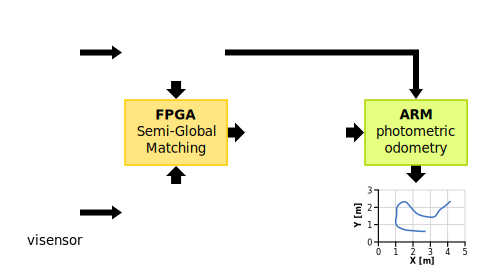
\includegraphics[width=\textwidth]{images/system_overview.pdf}
    \caption{schematic overview of the whole system}
    \label{fig:overview}
\end{figure}


The visensor provides a stream of frames, each of which consists of a stereo
pair of intensity data \footnote{Grayscale instead of full-color images are
used, because the information gain from colors is offset by the loss of
resolution. However, the approach described here would work similarly colors.}.

A semiglobal stereo matching core developed by [todo: ref] running on the FPGA
processes these and produces a disparity image which assigns every pixel the
disparity between the two cameras. The FPGA also provides a rectified camera
image.

This pair of intensity and disparity images is conceptually equivalent to a
three dimensional point-cloud, as we can calculate the distance to the camera
for every pixel from the disparity data. This is in turn makes it possible to
render the point-cloud from an arbitrary perspective, allowing us to look at an
image as if it was recorded from a different angle.

To estimate the ego-motion between two frames we can thus look for a
perspective that looks the same as the previous frame.  The movement of the
virtual camera will then correspond to the actual, physical movement of the
sensor.

By subtracting the intensities from the previous frame with the
intensities of the current frame sampled at the warped pixel locations a
photometric error is calculated, measuring the similarity of the warped current
frame with the previous one. The problem is now to minimize this error function.

Note that this approach assumes photoconsistency: Points have the same
intensity, regardless of viewing angle.


\section{Warping Pipeline}

\begin{figure}[h]
    \centering
    \includegraphics[width=\textwidth]{images/warp_pipeline.pdf}
    \caption{the full warping pipeline (pink pixels are not sampled by any of the warped points)}
    \label{fig:warp_pipeline}
\end{figure}

This section closely follows \cite{omaridenseodometry}.

Using an inverse projection derived from the standard pinhole camera model, a
point $ \vec{x} $ in the camera image plane can be back-projected into a point
$ \vec{p} $ in $ \mathbb{R}^3 $:

\begin{equation}
    \label{eq:backprojection}
    \vec{p} = \pi^{-1}(\vec{x}, D(\vec{x})) := \frac{b}{D(x)}
    \begin{bmatrix}
        \vec{x_u} - \vec{c_u} \\
        \vec{x_v} - \vec{c_v} \\
        f
    \end{bmatrix}
\end{equation}

where $b$ is the stereo baseline, $f$ the focal length and $\vec{c}$ the principal point of the camera.

This point $\vec{p}$ can now be moved into a new camera frame by translating and rotating it:

\begin{equation}
    \vec{p'} = \mat{T_R} \cdot \vec{p} + \vec{T_T}
\end{equation}

Where $T_R$ is a 3x3 rotation matrix and $T_T$ a three dimensional translation
vector. Using affine coordinates, we can write this as:

\begin{equation}
    \vec{p'} = \mat{T} \vec{p}
\end{equation}

A point in 3D space can be projected back onto the (now moved) camera image plane:

\begin{equation}
    \label{eq:projection}
    \vec{x'} = \pi(\vec{p'}) := \frac{f}{\vec{p'}_z}
    \begin{bmatrix}
        \vec{p'}_x \\
        \vec{p'}_y \\
    \end{bmatrix}
    + \vec{c}
\end{equation}

This whole warping operator can be summarized in a warping operator $\tau$:

\begin{equation}
    \vec{x'} = \tau(\vec{x}, D(\vec{x}), \vec{T}) := \pi( \mat{T} \cdot \pi^{-1} (\vec{x}, D(\vec{x})))
\end{equation}



\section{Minimization}

Using $\tau$, the error between the previous frame and the warped current frame can be defined as:

\begin{equation}
    e(\vec{x}, \vec{T}) := I_p(\tau(\vec{x}, \vec{T})) - I_c(\vec{x})
\end{equation}


To estimate the motion between two frames, this photometric error term should
be minimal for every pixel:

\begin{equation}
    \vec{\hat{T}} = \operatornamewithlimits{argmin}_{\vec{T}} \sum_{\vec{x} \in I_p} e(\vec{x}, \vec{T})^2
\end{equation}


This equation can be solved for the estimated motion by applying standard
optimization techniques, for exmple Gauss-Newton:

\begin{equation}
    \mat{J}^T \mat{J} \Delta \vec{T} = - \mat{J}^T \vec{e(\vec{T})}
\end{equation}

Here, $\mat{J} \in \mathbb{R}^{N \times 6}$ is the stacked Jacobian matrices
and $\vec{e(\vec{T})} \in \mathbb{R}^N$ the vector of the error terms of all
$N$ pixels.  This equation is iteratively solved for the increment $\Delta
\vec{T}$ of the motion estimation after recalculating the error term and
Jacobians from the new estimation.

The Jacobian is derived by applying the chain rule to photometric error term.
For a single pixel, we get a $1 \times 6$ Jacobian:

\begin{equation}
    \mat{J} := \mat{J_I} \mat{J_{\pi}} \mat{J_T}
\end{equation}

where $\mat{J_I} \in \mathbb{R}^{1 \times 2}$ is the image derivative of the warped previous frame and is
approximated using the image's gradient:

\begin{equation}
    \mat{J_I} := \frac{\partial \mathbf{I_p}(\vec{x})} {\partial \vec{x}} \bigg|_{\vec{x} = \tau(\vec{x}, \vec{T})}
    \approx
    \begin{bmatrix}
        \nabla{}_x \mathbf{I_p} & \nabla{}_y \mathbf{I_p}
    \end{bmatrix}
\end{equation}

The term $\mat{J_{\pi}}$ is the $2 \times 3$ Jacobian of the projection
function \ref{eq:projection}, evaluated at the warped 3D point:

\begin{equation}
    \mat{J_{\pi}} := \frac{\partial \pi(\vec{p})}{\partial \vec{p}}
    \bigg|_{\vec{p} = \vec{T}\cdot\pi^{-1}(\vec{x},\mathbf{D}(\vec{x}))}
    =
    \begin{bmatrix}
        \nicefrac{f}{\vec{p_z}} & 0 & -f \nicefrac{\vec{p_x}}{\vec{p_z}^2} \\
        0 & \nicefrac{f}{\vec{p_z}} & -f \nicefrac{\vec{p_y}}{\vec{p_z}^2}
    \end{bmatrix}
\end{equation}

$\mat{J_T}$ is the $3 \times 6$ Jacobian of the transformation operator $T$ and
the most costly term to compute:

\begin{equation}
    \mat{J_T} := \frac{\partial (\vec{T} \vec{p})}{\partial \vec{T}}
    \bigg|_{\vec{p} = \pi^{-1}(\vec{x}, \mathbf{D}(\vec{x}))}
\end{equation}
